\documentclass{scrartcl}
\usepackage{natbib}
\usepackage{amsmath, amsfonts, amssymb, bbm, graphicx}
\numberwithin{equation}{section}
\bibliographystyle{unsrtnat}

%opening
\title{Comparing Hamiltonian Monte Carlo and Elliptical Slice Sampling for constrained Gaussian distributions}
\subtitle{732A76 Research Project Report}
\author{Bayu Brahmantio (baybr878)}

\begin{document}

\maketitle

\section{Background}
High-dimensional multivariate gaussian distribution is used in various models and applications. In some cases, we need to generate from a certain distribution which applies constraints to a multivariate Gaussian distribution (\cite{gelfand1992GS} and \cite{RodrguezYam2004EfficientGS}). Sampling from this distribution is still a challenging issue, particularly because it is not straightforward to compute the normalizing constant for the density function.  

The gibbs sampler has proven to be a suitable choices to sample from truncated multivariate Gaussian distributions (\cite{gelfand1992GS}). Recently, more sophisticated methods have been developed to generate samples from truncated multivariate Gaussian distributions. In this research project, two methods, namely Exact Hamiltonian Monte Carlo (\cite{pakman2013exact}) and Analytic Elliptical Slice Sampling (\cite{Fagan2016ESSwEP}), will be compared. 


\section{Definitions}
\subsection{Truncated Multivariate Gaussian Distribution}
The truncated multivariate Gaussian distribution is a probability distribution obtained from a multivariate Gaussian random variable by bounding it under some linear (or quadratic) constraints.   

Let $\textbf{w}$ be a $d$-dimensional Gaussian random variable with mean vector $\boldsymbol{\mu}$ and covariance matrix $\boldsymbol{\Sigma}$. The corresponding truncated multivariate Gaussian distribution can be defined as
\begin{equation}\label{eq:tmg}
	p(\boldsymbol{\textbf{x}}) = \frac{\exp\{-\frac{1}{2}(\textbf{x}-\boldsymbol{\mu})^{\intercal} \boldsymbol{\Sigma}^{-1}(\textbf{x}-\boldsymbol{\mu})\}}{\int_{\textbf{F}\textbf{x} + \textbf{g} \geq 0} \exp\{-\frac{1}{2}(\textbf{x}-\boldsymbol{\mu})^{\intercal} \boldsymbol{\Sigma}^{-1}(\textbf{x}-\boldsymbol{\mu})\} d\textbf{x}}\mathbbm{1}(\textbf{F}\textbf{x} + \textbf{g} \geq 0)
\end{equation}
where $\textbf{x}$ is a $d$-dimensional truncated Gaussian random variable, $\mathbbm{1}$ is an indicator function, and $\textbf{F}$ is an $m \times d$ matrix, which, together with the $m \times 1$ vector of $\textbf{g}$, defines all $m$ constraints of $p(\boldsymbol{\textbf{x}})$.  We denote this as $\textbf{x} \sim TN(\boldsymbol{\mu}, \boldsymbol{\Sigma},\textbf{F},\textbf{g})$.   

We can rewrite $p(\boldsymbol{\textbf{x}})$ as
\begin{equation}\label{eq:tmg2}
	p(\textbf{x}) = \frac1Z\exp\bigg\{-\frac{1}{2}\textbf{x}^{\intercal} \boldsymbol{\Lambda} \textbf{x} + \boldsymbol{\nu}^{\intercal}\textbf{x}\bigg\}\mathbbm{1}(\textbf{F}\textbf{x} + \textbf{g} \geq 0)
\end{equation}
where $\boldsymbol{\Lambda} = \boldsymbol{\Sigma}^{-1}$, $\boldsymbol{\nu} = \boldsymbol{\Sigma}^{-1}\boldsymbol{\mu}$, and $Z$ is the normalizing constant. Through linear change of variables, \eqref{eq:tmg2} can be transformed into
\begin{equation}\label{eq:tmg3}
	p(\textbf{x}) = \frac1Z\exp\bigg\{-\frac{1}{2}\textbf{x}^{\intercal}\textbf{x}\bigg\}\mathbbm{1}(\textbf{F}^*\textbf{x} + \textbf{g}^* \geq 0)
\end{equation}
such that $\textbf{x} \sim TN(\textbf{0}, \textbf{I}_d,\textbf{F}^*,\textbf{g}^*)$, for some values of $\textbf{F}^*$ and $\textbf{g}^*$.









\subsection{Exact Hamiltonian Monte Carlo for Truncated Multivariate Gaussians}   
\subsubsection{Hamiltonian Monte Carlo}
Hamiltonian Monte Carlo (HMC) is a Markov Chain Monte Carlo method that makes use of an ideal system that follow Hamiltonian dynamics. A particle in this system can be described by a Hamiltonian energy function
\begin{equation}\label{eq:hml}
	H(\textbf{x}, \textbf{s}) = U(\textbf{x}) + K(\textbf{s})
\end{equation}
where $U(\textbf{x})$ is the potential energy term as a function of particle's position ($\textbf{x}$) and $K(\textbf{s})$ is the kinetic energy term as a function of particle's momentum ($\textbf{s}$). Both $\textbf{x}$ and $\textbf{s}$ are of $d$-dimensions.   
The change of position and momentum over time $t$ can be described by Hamilton's equations
\begin{equation}\label{eq:heqs}
\begin{split}
	\frac{\partial x_i}{\partial t} & = \frac{\partial H}{\partial s_i} \\
	\frac{\partial s_i}{\partial t} & = -\frac{\partial H}{\partial x_i}, \qquad i=1,...,d.\\
\end{split}
\end{equation}

To sample from a distribution using HMC, we can relate the target distribution to the current energy state of the particle through canonical distribution:
\begin{equation}\label{eq:can}
	p(\textbf{x}) \propto \exp\{-E(\textbf{x})\}
\end{equation}
where the target distribution, $p(\textbf{x})$, depends on the value of energy function $E(\textbf{x})$. In a Hamiltonian system, we have $H(\textbf{x}, \textbf{s})$ as our energy function, which results in the canonical distribution:
\begin{equation}\label{eq:can2}
\begin{split}
	p(\textbf{x}, \textbf{s}) &\propto \exp\{-H(\textbf{x}, \textbf{s})\} \\
	&\propto \exp\{-U(\textbf{x})\} \exp\{-K(\textbf{s})\} \\
	&\propto p(\textbf{x})p(\textbf{s}).
\end{split}
\end{equation}

Hence, $\textbf{x}$ and $\textbf{s}$ are independent. To sample from the target distribution $p(\textbf{x})$, we can sample from the joint distribution $p(\textbf{x}, \textbf{s})$ and ignore the variable $\textbf{s}$.  

\subsubsection{Exact HMC for Truncated Multivariate Gaussians}
Exact Hamiltonian Monte Carlo (HMC) for Truncated Multivariate Gaussians (TMG) (\cite{pakman2013exact}) considers the exact paths of particle trajectories in a Hamiltonian system that is proportional to the negative logarithm of TMG distributions density. Suppose our target distribution $p(\textbf{x})$ is a truncated multivariate Gaussian distribution as in ($\ref{eq:tmg3}$). We can set our momenta to be normally distributed, that is $\textbf{s} \sim \mathcal{N}(\textbf{0}, \textbf{I}_d)$. Therefore, the Hamiltonian system can be described as: 
\begin{equation}\label{eq:hsys}
	H = U(\textbf{x}) + K(\textbf{s}) = \frac{1}{2}\textbf{x}^{\intercal}\textbf{x} + \frac{1}{2}\textbf{s}^{\intercal}\textbf{s}
\end{equation}
subject to:  
\begin{equation}\label{eq:st}
	\textbf{F}\textbf{x} + \textbf{g} \geq 0.
\end{equation}
for some values of $\textbf{F}$ and $\textbf{g}$.   

The equations of motion for the Hamiltonian system in \eqref{eq:hsys} are:    
\begin{equation}\label{eq:heqs2}
\begin{split}
	\frac{\partial x_i}{\partial t} & = \frac{\partial H}{\partial s_i} = s_i \\
	\frac{\partial s_i}{\partial t} & = -\frac{\partial H}{\partial x_i} -x_i, \qquad i=1,...,d.\\
\end{split}
\end{equation}

In this sense, we want the particles in Hamiltonian system to only move around inside the constrained space. The exact trajectory of a particle using the equations above is:    
\begin{equation}\label{eq:path}
	x_i(t) = s_i(0)\sin(t) + x_i(0)\cos(t).
\end{equation}

A particle will follow the trajectory above until it hits a wall, or in other words, until $\textbf{F}\textbf{x} + \textbf{g} = 0$. Let $t_h$ be the time when the particle hits wall $h$, or when $\textbf{F}_h \cdot \textbf{x}(t_h) + \text{g}_h = 0$. It will hit the wall with velocity $\dot{\textbf{x}}(t_h)$ which can be decomposed into:   
\begin{equation}\label{eq:bounce}
	\dot{\textbf{x}}(t_h) = proj_{\textbf{n}}\dot{\textbf{x}}(t_h) + proj_{\textbf{F}_h}\dot{\textbf{x}}(t_h)
\end{equation}
where $proj_{\textbf{n}}\dot{\textbf{x}}(t_h)$ is the projection of $\dot{\textbf{x}}(t_h)$ on the normal vector $\textbf{n}$ perpendicular to $\textbf{F}_h$ and
\begin{equation}\label{eq:proj}
\begin{split}
	proj_{\textbf{F}_h}\dot{\textbf{x}}(t_h) &= \frac{\textbf{F}_h \cdot \dot{\textbf{x}}(t_h)}{||\textbf{F}_h||}\frac{\textbf{F}_h}{||\textbf{F}_h||}\\  
	&= \frac{\textbf{F}_h \cdot \dot{\textbf{x}}(t_h)}{||\textbf{F}_h||^2}\textbf{F}_h \\
	&= \alpha_h\textbf{F}_h.
\end{split}
\end{equation}
By inverting the direction of $proj_{\textbf{n}}\dot{\textbf{x}}(t_h)$, we can obtain the reflected velocity as
\begin{equation}\
\begin{split}
	\dot{\textbf{x}}_R(t_h) & = -proj_{\textbf{n}}\dot{\textbf{x}}(t_h) + proj_{\textbf{F}_h}\dot{\textbf{x}}(t_h) \\
	& = -\dot{\textbf{x}}(t_h) + 2\alpha_h\textbf{F}_h
\end{split}
\end{equation}
which can be used as the new initial velocity ($s_i(0)$) in \eqref{eq:path} for the particle to continue its path. It can be shown that exact HMC follows the detailed balanced condition (\cite{pakman2013exact}) which leaves the canonical distribution invariant.    

The process of sampling using exact HMC can be summarized into two steps:   
\begin{enumerate}
	\item Sample $\textbf{s}$ from $\mathcal{N}(\textbf{0}, \textbf{I}_d)$.
	\item Use $\textbf{s}$ and the last value of $\textbf{x}$, and move the particle for a time $T$ until we reach $\textbf{x}^*$ and $\textbf{s}^*$. Use $\textbf{x}^*$ as initial positions for the next iteration.
\end{enumerate}

\subsection{Analytic Elliptical Slice Sampling}   
\subsubsection{Slice Sampling}
Slice sampling (\cite{Neal2003}) is a method that tries to sample uniformly from the ($n+1$)-dimensional region under $f(x)$ that is proportional to density function$p(x)$. It is done by using Gibbs sampling to sample from the joint distribution $(x, y)$ where $y$ is an auxiliary variable. We do this by alternately sampling from $y|x \sim \text{U}(0, f(x))$ and $x|y \sim \text{U}(S)$ where $S = \{x: f(x)>y\}$. To obtain samples from $x$, we can sample from $p(x,y)$ and ignore the $y$ later.   

\subsubsection{Elliptical Slice Sampling}
Elliptical slice sampling (ESS, \cite{murray2010}) is a form of slice sampling that uses Gaussian prior to sample from a posterior distribution of the form
\begin{equation}\label{eq:ESSpost}
	p^*(\textbf{x}) = \frac1Z\mathcal{N}(\textbf{x};\textbf{0}, \boldsymbol{\Sigma}) L(\textbf{x})
\end{equation}
where $Z$ is the normalization constant, $\mathcal{N}(\textbf{0},\boldsymbol{\Sigma})$ is a multivariate Gaussian prior, and $L$ is a likelihood function. To do this, we introduce an auxiliary variable $\boldsymbol{\nu} \sim \mathcal{N}(\textbf{0}, \boldsymbol{\Sigma})$ so that given an initial state $\textbf{x}$, the update ellipse is   
\begin{equation}\label{eq:rule}
	\textbf{x}' = \textbf{x}\cos(\theta) + \boldsymbol{\nu}\sin(\theta), \quad  \theta \in [0, 2\pi]
\end{equation}   

The algorithm begins by sampling the slice height $y \sim \text{U}(0, L(\textbf{x}))$ and the auxiliary variable $\boldsymbol{\nu} \sim \mathcal{N}(\textbf{0}, \boldsymbol{\Sigma})$ that determines the ellipse in \eqref{eq:rule}. We then sample $\theta$ uniformly from $[0, 2\pi]$ and shrink the interval towards $\theta=0$ (initial state) until we found $\theta$ that satisfies $L(\textbf{x}') > y$. The new point is accepted as the next state and we use it as the initial state for the next iteration.   

ESS is analogous to slice sampling in the sense that it samples uniformly from the height of function and from the interval where the function value is more than the height. Furthermore, it can be shown that the transition operator of ESS is reversible which implies that the Markov chain converges to the target posterior distribution (\cite{murray2010}).   

\subsubsection{Analytic Elliptical Slice Sampling}
Analytic Elliptical Slice Sampling (\cite{Fagan2016ESSwEP}) tries to cut the process of shrinking the ellipse in ESS by pre-determining the possible sampling interval. First, we define
\begin{equation}\label{eq:ellipse}
	\mathcal{E} = \{\textbf{x}':\textbf{x}'(\theta) = \textbf{x}\cos(\theta) + \boldsymbol{\nu}\sin(\theta)\}
\end{equation} 
as the set of possible new states and define
\begin{equation}\label{eq:slice}
	\mathcal{S}(y,\mathcal{E}) = \{ \textbf{x}'\in \mathcal{E}: L(\textbf{x}')>y\}
\end{equation}
as the slice of acceptable proposed state. To form a markov chain that converges to the posterior distribution, we need to sample uniformly from the analytically pre-determined slice $\mathcal{S}(y,\mathcal{E})$ (\cite{Fagan2016ESSwEP}). That is, the algorithm is similar to ESS except that the process of shrinking the ellipse is replaced by determining $\mathcal{S}(y,\mathcal{E})$ so that sampling from $\theta$ guarantees to yield a new state $\textbf{x}'$.    

In a truncated multivariate Gaussian setting, we have
\begin{equation}\label{eq:tmgESS}
\begin{split}
	p^*(\textbf{x}) &= \frac1Z\mathcal{N}(\textbf{x};\textbf{0}, \boldsymbol{\Sigma}) TN(\textbf{x};\textbf{0},\textbf{I}_d,\textbf{F},\textbf{g}) \\
	&\propto \mathcal{N}(\textbf{x};\textbf{0},\boldsymbol{\Sigma}) \mathcal{N}(\textbf{x};\textbf{0},\textbf{I}_d)\mathbbm{1}(\textbf{F}\textbf{x} + \textbf{g}\geq 0)
\end{split}
\end{equation}
Given $\textbf{x}$, $\boldsymbol{\nu}$, and $y$, we can determine the slice of possible new states as
\begin{equation}\label{eq:exactslice}
\begin{split}
	\mathcal{S}(y,\mathcal{E}) &= \{\theta \in [0,2\pi]:  L(\textbf{x}')>y\} \\
	&= \cap^m_{j=1}\ \{\theta \in [0,2\pi]: F_j^{\intercal}\textbf{x} + g_j \geq0 \} \\
	& \quad \cap\{\theta \in [0,2\pi]: \mathcal{N}(\textbf{x};\textbf{0},\textbf{I}_d)>y\}.
\end{split}
\end{equation}   

\cite{Fagan2016ESSwEP} also demonstrates how to sample $J$ points from a single ESS iteration. In an ESS setting, it is done by 'recycling' the interval that has been sampled until $J$ points are accepted. One of the $J$ points is then randomly selected as the next initial state. In the case of analytic ESS, $J$ different values of y are sampled and for each of them we find the corresponding $\mathcal{S}(y,\mathcal{E})$ and uniformly sample one point.   


\section{Results}
In this section we are going to compare both methods (Exact HMC for TMG and Analytic ESS) under different settings of truncated multivariate gaussians.

Figure 1 shows how both algorithms sample a two-dimensional gaussian distribution with some constraints that results in a narrow support, similar to Figure 1 in \cite{pakman2013exact}. From both cases, we can see that they worked as expected. The generated samples rapidly converged to the mean while also complying the constraints.     


\begin{figure}[h!]
	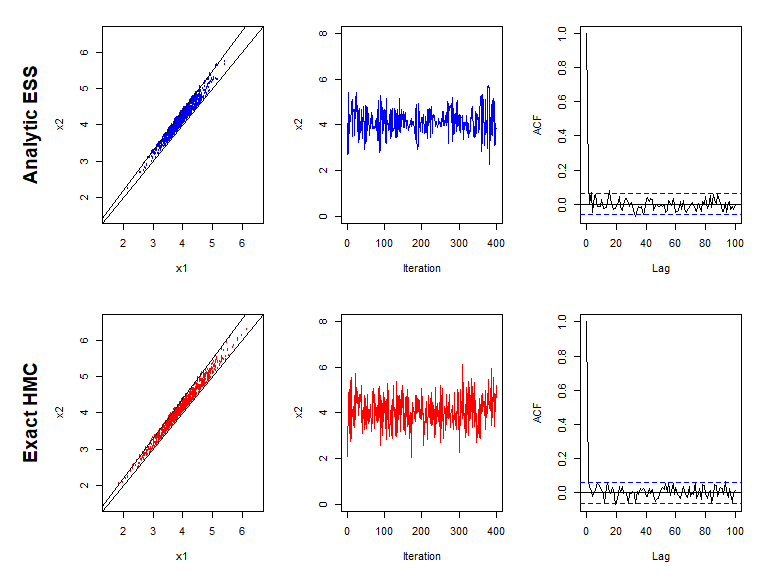
\includegraphics[width=\linewidth]{fig1.png}
	\caption{Comparison of generated points from $\mathcal{N}((4,4)^T,\textbf{I}_2)$ under the constraints $x_1 \leq x_2 \leq1.1 x_1$ and $x_1,x_2 \geq 0$ with initial points (2, 2.1). First column: 1000 iterations. Second column: trace plots of the first 400 iterations of $x_2$. Third column: Autocorrelation of $x_2$. In this example we used $T=\pi/2$ for HMC and $J=1$ for ESS. Both methods converges around $x_2=4$ and have relatively low autocorrelation scores.}
\end{figure}

Notice that the maximum traveling time $(T)$ and number of samples per iteration $(J)$ affect the computation time for Exact HMC and Analytic ESS respectively. The higher the maximum traveling time ($T$), the longer it takes for a particle in an HMC system to move while also increases the possibility of bouncing. At the same time, an increase in the value of $J$ lets us sample multiple points from the same ellipse without a significant increase in computation time.    


From the experiments, we observed a large disparity between the runtimes of both algorithms. As seen in the Table 1, Exact HMC performs much faster than the fastest Analytic ESS.     


\begin{table}
\centering
\begin{tabular}{|c|c|}
	\hline
	Method & Avg. computation time per sample (second) \\
	\hline
	HMC($T=\frac{\pi}{2}$) & 0.0001728 \\
	\hline
	HMC($T=\frac{3\pi}{4}$) & 0.000173 \\
	\hline
	ESS($J=1$) & 0.0271275 \\
	\hline
	ESS($J=5$) & 0.0250084 \\
	\hline
	ESS($J=10$) & 0.0236001 \\
	\hline
\end{tabular}
\caption{Average computation time per sample for both models under different settings for 10-dimensional TMG under the constraints $-1 \leq x_i \leq 1, i=1,...,10$ using CPU. For HMC, T is the maximum travel time. For ESS, J is the number of points sampled in each iteration. The computation time for Exact HMC is overall much faster than Analytic ESS.}
\end{table}


\section{Discussion}
In this research project, we have compared Exact HMC and Analytic ESS. In terms of the generated samples, they are not significantly different. Exact HMC also performs much faster than Analytic ESS. More rigorous measurements can be made to evaluate whether the samples are autocorrelated within a chain or not by measuring their effective sample size.     

There are, however, some caveats to the computation of Analytic ESS in this case. We expected the runtime to be somewhat similar to Exact HMC, but it runs more than 100 times slower. This could be to the fact that external packages are used for the computation of the intervals and slices which could have been replaced by customized functions that are more specific to the task, hence the faster runtime. The programming language used $\texttt{R}$ is also not popularly chosen because of its speed. Thus, the algorithm might need to be rewritten in a language that is proven to be computationally faster (e.g. $\texttt{Python}$).   


\newpage
\bibliography{ref}

\end{document}
